\documentclass[a4paper,10pt]{article}
\usepackage{hcolor}
\usepackage{color}
\usepackage{fancyhdr}
\usepackage[pdftex]{graphicx}

\def\RCS$#1: #2 ${\expandafter\def\csname RCS#1\endcsname{#2}}
\RCS$Date$
\RCS$Revision$


\setlength\topmargin{0in}
\setlength\headheight{0in}
\setlength\headsep{0.2in}
\setlength\textheight{24cm}
\setlength\textwidth{6.5in}
\setlength\oddsidemargin{0in}
\setlength\evensidemargin{0in}
\setlength\parindent{0.25in}
\setlength\parskip{0.25in}


\newcommand{\code}[1]{%
\begin{center}
  \fboxsep=10pt
  \fcolorbox{black}{green}
  {
       \parbox[c]{12cm}{
     \color{blue}{#1}}
  }
\end{center}}


% Title Page
\title{BankEfficiency documentation}
\author{Thomas Cokelaer}

\begin{document}
\bibliographystyle{unsrt}
\pagestyle{plain}
\fancypagestyle{plain}
\rfoot{}
\cfoot{\arabic{page} of \pageref{theend}}
\lfoot{}
\pagestyle{plain}
\lhead{BankEfficiency documentation -- v.\RCSRevision, \RCSDate}



\maketitle
\section{Introduction}

BankEfficiency is a tool, which is available in lalapps/src/findchirp, that was primarely created to test efficiencies of template banks at detecting inspiralling compact binaries in the context of ground based detetectors. 

Although it relies heavily on LAL packages such as bank, inspiral and noisemodels packages, nevertheless it has its own sets of routines, which makes BankEfficiency a pretty long piece of code (about 4,000 lines) but also quite independant. BankEfficiency is quite modular, and the main core is pretty small (about 400 lines). It should therefore be easy to adapt it to your needs. 

\textbf{What BankEfficiency can do :}
\begin{itemize}
 \item Compute overlaps between a signal and a template bank
 \item Perform large Monte-Carlo simulations using condor and dag technology.
 \item Store results in XML format both for data mining and keep track of the parameters being used.
 \item Inject any type of signal that is available in LAL inspiral package
 \item Use any template bank that is available in LAL bank package
 \item Use any noise model that is available in LAL noisemodel package
\end{itemize}

\textbf{What BankEfficiency cannot do }
\begin{itemize}
 \item a multidetector anaylis
 \item analyse real noise, although implementation of an interface should be straigtforward.
 \item PTF filtering
 \item BCV spin filtering
\end{itemize}

BankEfficiency has become a powerful tool but it neccesiates a lot of input arguments, most of them having default values hardcoded. The documentation has two main objectives that are (1) explain what type of simulations you can performed with BankEfficiency, and (2) how to set the input parameters properly.

In the following we assume that the reader knows what is a template bank, what is matched filtering, what is a template, and what are the models such as EOB, PadeT1, TaylorT1 and so on. If not, you may look at one of the references in the bibliography 

\section{Tutorial}
In this section, I will introduce a few examples to show what type of simulations BankEfficiency and what is the ouput. 

\subsection{First example and outputs}
Let us start with a very simple example that has only two input parameters. This is possible because all parameters have default values. 

\code{lalapps\_BankEfficiency {-}{-}template EOB {-}{-}signal EOB}

Here, we specify both the signal and templates model to be based on EOB model. To do so, we use (\textbf{{-}{-}signal EOB}) and (\textbf{{-}{-}template EOB}). The code will inject an EOB signal and filter it trough a template bank whose templates are also based on EOB signal. We'll come back on the template bank placement later on. This command returns a bunch of numbers on the screen. 

The next step is to understand what all these numbers are. From the output on the screen this is quite tedious. Luckily, at the end of the previous command, one can add \textbf{--xml-output}:

 \code{lalapps\_BankEfficiency {-}{-}template EOB {-}{-}signal EOB {-}{-}xml-output}

This option will create a file called \textbf{BankEfficiency-Result.xml} that contains (1) all the input parameters and (2) all the results of the simulation.

Here, we assume that you are familiar with \textbf{lwtprint} executables from ligotools. The output results of BankEfficiency are stored in XML format in a table that is called \textbf{bankefficiency}. From now, you can extract the output of BankEfficiency using this kind of command: 

\code{lwtprint BankEfficiency-Result.xml -t bankefficiency -c mass1\_sim,mass2\_sim,snr}

where \textbf{-t bankefficiency } parses the bankefficiency outputs and \textbf{-c snr,mass1\_sim,mass2\_sim} means you want to extract the columns labelled \textbf{snr}, \textbf{mass1\_sim} and \textbf{mass2\_sim}. Of course, you need to know what are the column's name. At the end of this document, we provide the list of columns and their meaning 

In the previous example, we extracted the component masses as well as the SNR. Actually, this is the overlap between the signal and the template bank that is a single number for each injected signal. This single number is therefore a maximisation over time and parameter space of all the correlation/matched filtering performed during a simulation.

As you've probably noticed, the input parameters can be very succint. In this first example, we provide only 2 or 3 arguments. This simply means that many parameters are set by default. For instance the sampling is 2048Hz and  the template bank is based on a square placement. In order to know all the default values, you can consult the header of BankEfficiency. A nicer way is again to look at the XML file. Indeed, all the parameters used for the simulation are stored in the \textbf{process\_params} table togethre with the version of the code that has been used stored in \textbf{process} table, you should be able to reproduce your results. Finally, if you use \textbf{BankEfficiency} as a standalone and add the option \textbf{--print-bank}, you will also have the template bank stored in a file called \textbf{BankEfficiency-Bank.xml}.



\subsection{Second example: testing a template bank}
What you want to do to test that a template bank is well designed is large number of simulations. The number of simulations can be specified with \textbf{--n 10000}. 

Then, to be realistic, the minimal match of the bank is set to \textbf{-- mm 95\%} (by default it is set to 80\%).

\code{lalapps\_BankEfficiency {-}{-}template EOB {-}{-}signal EOB {-}{-}mm 0.95 {-}{-}n 10000  {-}{-}xml-output {-}{-}print-bank}

Finally, what you really want to look at is some plots. BankEfficiency does not create any plots for you. So you can use whatever tool you prefer. however, within lalapps/src/findchirp package, there are 2 python files called plotbankefficiency.py and inspiraltools.py. Use the former one as follows : 

\code{python plotbankefficiency.py --glob 'BankEfficiency-Results.xml' --verbose --user-tag 'test'} so as to generate a bunch of plots you may found useful. For instance, Fig.\ref{fig:snr1} shows the distribution of the overlaps versus total mass.

\begin{figure}
\centering
 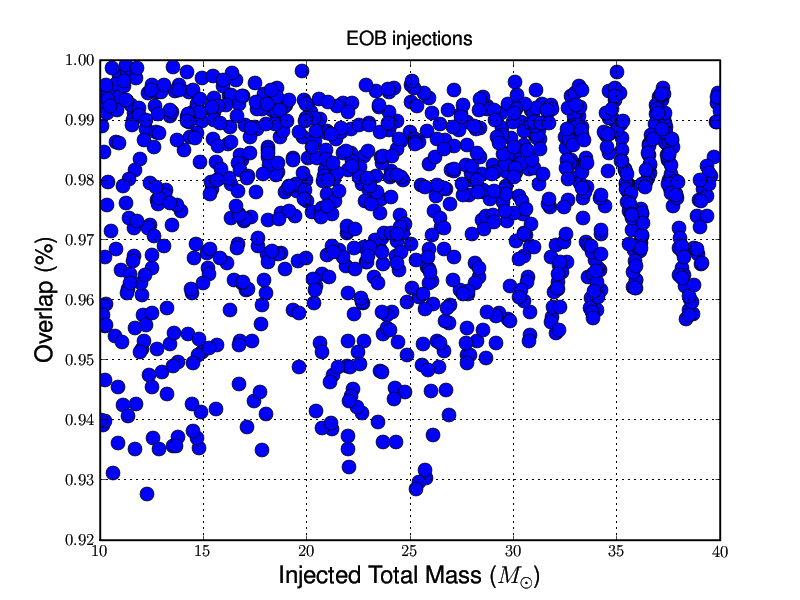
\includegraphics[width=0.4\textwidth]{bankefficiencydoc_snr_versus_totalmass.png}
\caption{\label{fig:snr1} Overlaps versus total mass}
\end{figure} 

Note that the XML table does not contains all the physical information you may want. For instance, it contains only the component masses of the injected waveform but the chirp mass or eta are not there. you can compute it afterwards. So, it is not stored to save disk space.

\subsection{Third example: noise and signal}
In the two previous examples, we consider noiseless simulations. BankEfficienc was indeed crated to check the overlap betweem template bank and an injection. But, thanks to the noisemodel package, it is straightforward to use simulation where the signal is buried in some noise. This can be done as follows : 
\code{lalapps\_BankEfficiency {-}{-}template EOB {-}{-}signal EOB {-}{-}mm 0.95 {-}{-}n 10000  {-}{-}xml-output {-}{-}print-bank  {-}{-}simulation-type NoiseAndSignal --signal-amplitude 25}

The noise is a colored gaussian noise with a variance such that the average SNR is set by \textbf{{-}{-}signal-amplitude} to 25. 

This is very useful to perform test of the Fisher matrix by testing the dispersion/accuracy of the mass parameters. 

Usually, you would want the mass of the injection to be fixed instead  of being randomized. This can be done by fixing the individual masses as follows: 
\code{lalapps\_BankEfficiency {-}{-}template EOB {-}{-}signal EOB {-}{-}mm 0.95 {-}{-}n 10000  {-}{-}xml-output {-}{-}print-bank  {-}{-}simulation-type NoiseAndSignal {-}{-}signal-amplitude 25 {-}{-}m1 10 {-}{-}m2 10}

Another option related to the noise is that you may want to specify different type of colored noise, which currently are LIGOI, LIGOA, VIRGO, EGO, TAMA for initial LIGO, advanced LIGO, VIRGO, Einstein Telescope and TAMA, which can be fixed by \textbf{{-}{-}noise-model}.


\code{lalapps\_BankEfficiency {-}{-}template EOB {-}{-}signal EOB {-}{-}mm 0.95 {-}{-}n 10000  {-}{-}xml-output {-}{-}print-bank  {-}{-}simulation-type NoiseAndSignal {-}{-}signal-amplitude 25 {-}{-}m1 10 {-}{-}m2 10 {-}{-}noise-model LIGOA}

using the --print-psd option, the PSD will be saved in \textbf{BankEfficiency-PSD.dat}.

\section{Reference}

\subsection{template bank related}
ffinal,
compute moments
hexagonal, squareNotOriented
mm 
fine bank
see BCV for bcv related
\subsection{Eccentricity related}
ecc-range
\subsection{standard time domain models (TaylorT1, EOB...)}
order
\subsection{BCV related functions}
no-alpha-constraint
alpha-constraint
alpha
psi0
bank-fcut range
bank-alpha
see BCV reference
\subsection{Amplitude Corrected related}
amp-order

\subsection{others}
num-seconds
fast option  and e-match
sampling
seed
bhns-injection
check/faithfulness
print-snr-histo

\section{Using BankEfficiency with DAG and condor on a cluster}
\subsection{ini file}
fix your ini file so that it does what you want.
\subsection{Generate the sub abd dag files.}
python bep.py --config-file bep.ini
creates bep.dag
run your simulation

\section{Meaning of the bankefficiency XML table}
\begin{description}
\item[psi0] The first BCV parameter of the template
\item[psi3] The second BCV parameter of the template
\item[psi0\_sim] The first BCV parameter of the injection
\item[psi3\_sim] The second BCV parameter of the injection
\item[tau0] The first mass parameter of the template
\item[tau3] The second mass parameter of the template
\item[tau0\_sim] The first mass parameter of the injection
\item[tau3\_sim] The second mass parameter of the injection
\item[ecc] eccentricity of the best templates
\item[ecc\_sim] eccentricity of the signal
\item[ffinal] ffinal of the best templates
\item[ffinal\_sim] ffinal of the injection
\item[mass1\_sim] The first mass parameter of the injection
\item[mass2\_sim] The first mass parameter of the injection
\item[phase\_sim] The initial phase of the injection
\item[snr] the best overlap maximised over all template bank and time
\item[snr\_at\_ta] irrelevant for now
\item[phase] the phase of the best template
\item[alpha\_f] the alpha\_f value of the best template (BCV related)
\item[time] the time of arrival of the best template
\item[time\_sim] 
\item[nfast] number of templates really used
\end{description}

\section{The options and their default values}




% bibliography : bank papers : square, hexa, bcvspin, S3SBBH, reinhard, owen, Sathya,
\begin{thebibliography}{99}
\bibitem{LIGO}
A. Abramovici {\it et al.}, Science {\bf 256}, 325 (1992);
B. Abbott, {\it et al.}, Nuclear Inst. and Methods in Physics 
Research, A {\bf 517/1-3} 154 (2004).

\bibitem{VIRGO}
B. Caron {\it et al.}, Class. Quantum Grav. {\bf 14}, 1461 (1997);
F. Acernese {\it et al.}, {\em The Virgo detector,} 
Prepared for 17th Conference on High Energy Physics (IFAE 2005) (In Italian), 
Catania, Italy, 30 Mar-2 Apr 2005,  AIP Conf. Proc. {\bf 794}, 307-310 (2005).

\bibitem{damir}
F.~Beauville et al, Class.\ Quant.\ Grav.\ \textbf{22}, 4285, (2005).

\bibitem{Owen96}B.~Owen, Phys.\ Rev.\  D\textbf {53}, 6749 (1996).

\bibitem{OwenSathyaprakash98} B.~Owen, B.~S.~Sathyaprakash 1998 Phys.\ Rev.\ 
D \textbf{60} 022002 (1998).

\bibitem{squarebank}
S.~Babak and R.~Balasubramanian and D.~Churches and T.~Cokelaer and B.~S.~Sathyaprakash 2006 \textit{Class.\ Quantum Grav.\ }
\textbf{23} 5477

\bibitem{hexabank} T.~Cokelaer 2007 \textit{Gravitational Wave Detections of Inspiralling Compact Binaries: Hexagonal Template Placement and Physical Template Families}, (\textit{Preprint} gr-qc/0706.4437v1), Phys. Review D 76, 10, 2007 (15 Nov 2007) 


\bibitem{bcvbank} T.Cokelaer, 2007, \textit{A template bank to search for gravitational waves from inspiralling compact binaries: II. Phenomenological model}
Class. Quantum Grav. 24 (2007) 6227-6242 


\bibitem{BDI95} L. Blanchet, T. Damour and B.R. Iyer, Phys.\ Rev.\ D {\bf 51},5360 (1995).

\bibitem{LAL} LSC Algorithm Library LAL,\\
{\tt http://www.lsc-group.phys.uwm.edu/daswg/\-projects/lal.html}

\bibitem{LIGOS3S4}
B.~Abbott {\it et al.}, LIGO Scientific Collaboration, gr-qc/0704.3368v2,
(2007)

\bibitem{PSDs}
T.~Damour and B.R.~Iyer and B.S.~Sathyaprakash, Phys.\ Rev.\ D
\textbf{63}, 044023 (2001).

\end{thebibliography}


\label{theend}

\end{document}          

